\section{Tarea}
\begin{itemize}
    \item Elabore un informe paso a paso de la implementación una Trie para insertar, buscar y reemplazar palabras en un texto.
    \item Utilice interfaces gráficas de usuario para su implementación.
    \item Utilice todas las recomendaciones dadas por el docente.
    \item Utilice la siguiente GUI como referencia:
    \begin{figure}[h!]
        \begin{center}
            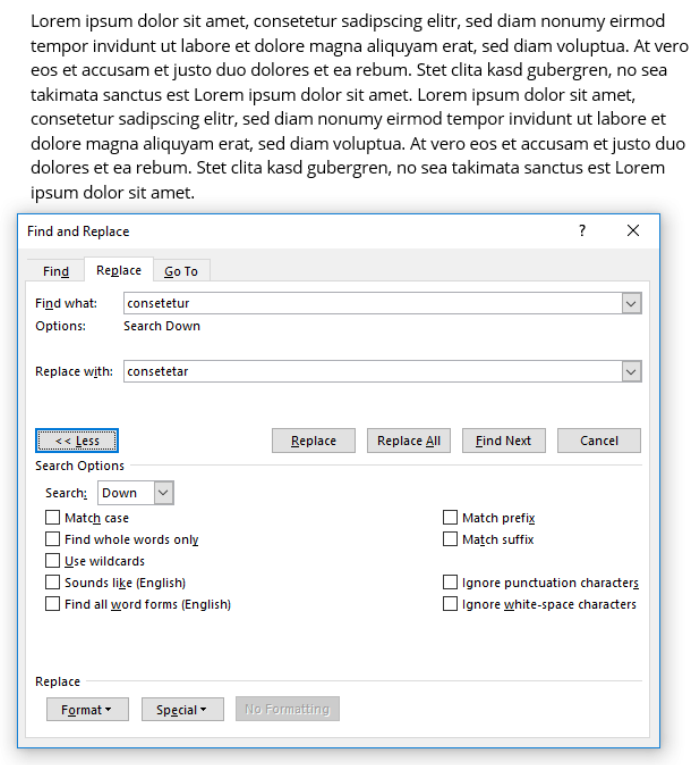
\includegraphics[scale=0.28]{img/GUI.png}
        \end{center}
    \end{figure}
\end{itemize}
\section{URL de Repositorio Github}
\begin{itemize}
    \item URL del Repositorio GitHub para clonar o recuperar.
    \item \url{https://github.com/DiegoNiS/Laboratorio-EDA-Colab.git}
\end{itemize}


% \section{Ejecuciones}


%\clearpage
\section{Pregunta}
\textbf{Explique. ¿Cómo se utiliza esta estructura de datos para almacenar prefijos?.}\\



\section{Pregunta}
\textbf{Explique. ¿Cómo se utiliza esta estructura de datos para almacenar prefijos?.}\\

